%!TEX root = ../rapport.tex

\chapter{Phase de tests avancée}
La phase de tests dite avancé va introduire la Set-Top Box ainsi que l'implémentation du client et du serveur pour un fonctionnement final. Nous aurons donc l'introduction des Web Services sur le serveur.

La situation est la suivante:

\medskip

J'utilise un switch, où sont connectés mon ordinateur, qui fait office de serveur, la Set-Top Box ainsi qu'un routeur. Les adresses IP sont ainsi distribuées via DHCP par le routeur.

\begin{figure}[H]
      \centering
      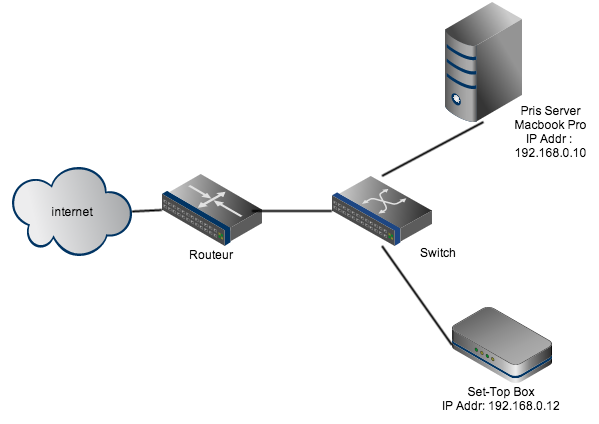
\includegraphics[width=\textwidth]{00_media/env_avance}
      \caption{Environnement de développement avancé}
      \label{gra:maqmenu}
\end{figure}
\section{Conception}

\subsection{Identification de la Set-Top Box}
Chaque Set-Top Box est identifiable par sa MAC adresse. Lorsqu'une Box se connectera sur notre serveur, la première valeur qui sera envoyée vers celui-ci est sa MAC adresse. De plus, cette information est disponible sur Thom.

\medskip

Ainsi, il sera possible de répertorier et identifier chaque session par la MAC adresse, en imaginant une table ayant pour clé l'adresse et la session comme objet. Lorsque l'adresse a été ajoutée avec la session, la communication est établie et le dialogue peut commencer.

\begin{figure}[H]
      \centering
      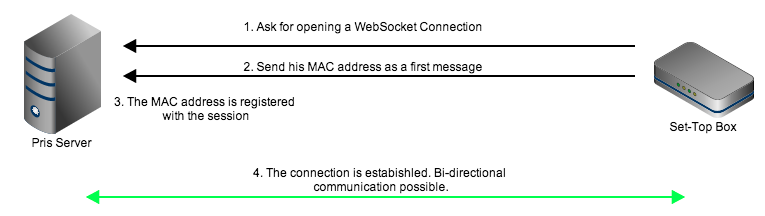
\includegraphics[width=\textwidth]{00_media/connection}
      \caption{Démarrage de la Set-Top Box}
      \label{gra:maqmenu}
\end{figure}

\medskip

Nous utiliserons une \textbf{HashTable} dont la clé sera de type \textbf{String}, pour l'adresse MAC et la valeur sera de type \textbf{Session} pour stocker la session distante.
\subsection{Centralisation des WebSockets}
Afin de faciliter la communication entre les Web Services et les WebSockets, une classe passerelle sera créée. Car bien qu'il s'agisse du même serveur, il faut pouvoir transférer les requêtes reçues vers la partie WebSockets.

\medskip

Le but est donc d'avoir une classe singleton, qui contiendra notre HashTable. Elle contiendra deux méthodes, \textbf{join} et \textbf{leave}, qui permettent respectivement d'ajouter une session dans la HashTable et de la retirer lorsque la connexion est fermée. De plus, chaque service aura sa méthode dans cette classe. Lorsque le Web Service recevra une requête, il la transmettre à notre WebSocketCentralisation, qui elle la transmettra au bon Socket, qui pourra communiquer avec la STB.

\medskip

C'est elle aussi qui retourna la valeur de retour au Web Service, qui pourra à son tour retourner la valeur au demandeur.

\begin{figure}[H]
      \centering
      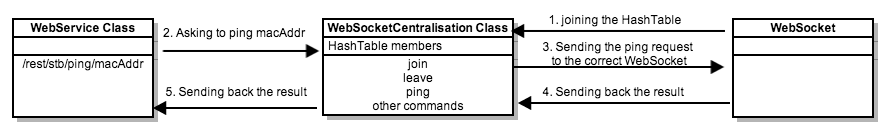
\includegraphics[width=\textwidth]{00_media/websocketCentr}
      \caption{Fonctionnement de la WebSocketCentralisation}
      \label{gra:maqmenu}
\end{figure}

\subsection{Envoi de commandes sur la Set-Top Box}

En complément de ce qui a été vu précédemment, nous allons définir le déroulement d'un envoi d'une commande en partant de Thom, jusqu'à notre Set-Top Box et le retour des données.

\medskip

\begin{enumerate}
	\item Pour commencer, Thom fait une requête à l'adresse du Web Service désiré.
	\item Réception faite, Pris envoie la requête à la STB au format JSon.
	\item La STB réceptionne la requête, exécute la commande, puis retourne le résultat, au format JSon, sur Pris.
	\item Pris réceptionne le résultat et le retourne, toujours au format JSon, vers Thom.
\end{enumerate}

\begin{figure}[H]
      \centering
      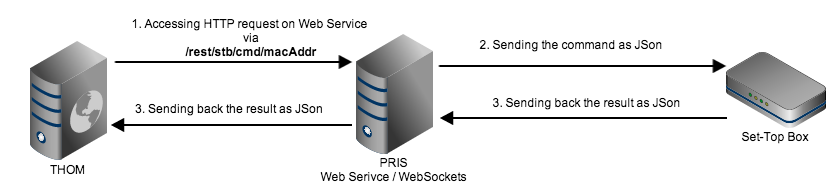
\includegraphics[width=\textwidth]{00_media/sending_cmd}
      \caption{Envoi de commande depuis Thom}
      \label{gra:maqmenu}
\end{figure}

\medskip

Comme le montre la figure ci-dessus, les données transitées sont au format JSon. Il sera ainsi possible via un seul String de définir de quel type de commande il s'agit, et de transmettre des informations supplémentaires, par exemple pour un ping, choisir la destination. Voici un exemple de JSon représentant le résultat d'un ping.

\begin{lstlisting}[caption={Résultat au format JSon}]
{
  "type" : "ping",
  "data_size_unit" : "bytes",
  "time_unit" : "ms",
  "ip_dest" : "173.194.35.24",
  "macAddr" : "00:09:DF:1B:FC:A5",
  "data_size" : 64,
  "packet_loss" : 0.0,
  "time" : 35.2,
  "round_trip_avg" : 35.236,
  "round_trip_max" : 35.236,
  "round_trip_min" : 35.236,
  "round_trip_stddev" : 0.0,
  "packet_transmitted" : 1,
  "icmp_seq" : 1,
  "ttl" : 52,
  "packet_received" : 1
}

\end{lstlisting}

Voici un JSon représentant une requête de ping envoyée sur la Set-Top Box
\begin{lstlisting}[caption={Résultat au format JSon}]
	{
		"opt":"google.ch",
		"cmd":"ping"
	}
\end{lstlisting}

"cmd" étant la commande à effectuer et "opt" les options possibles de ping. Ici il s'agit juste de la destination.
\subsection{Synchronisation des données}
Un problème persiste, comment synchroniser le retour des données de la Set-Top Box jusqu'au Web Service, sachant que je n'ai aucun moyen de savoir, lorsque j'envoie la requête via WebSockets sur la box, quand le résultat va m'être retourné.

\medskip

Il existe un sous-protocole des WebSockets, nommé \textbf{The WebSocket Application Messaging Protocol} (WAMP). Ce que permet de faire WAMP est d'appliquer le principe de \textbf{Publish and Subscribe}, qui permet de s'inscrire sur un serveur pour recevoir des notifications, ce qui ne nous intéresse pas, et le principe de \textbf{Remote Procedure Call}(RPC). Ici, cela devient plus intéressant, car il s'agit d'appeler des méthodes et d'avoir un \textbf{callback}, c'est-à-dire que lorsque l'appel de méthode à distance est fini, le résultat est envoyé et nous pouvons \textbf{attendre} sur celui-ci. Le problème est que l'appel de méthode se fait sur ... le serveur! Or, ce que nous aurions aimé, c'est faire appel au client.

\medskip

J'ai toute fois utilisé le même principe. Lorsque le Socket envoie la commande à la STB, celui-ci va attendre sur le résultat. Tant que le résultat attendu est vide, j'attends. Dès que le résultat est arrivé, je le renvoie au demandeur.

Nous pouvons faire un \textbf{sleep} du Thread courant, qui permettra d'attendre que le résultat soit mis à jour. Si ce n'est toujours pas le cas, je le rendors.


\begin{figure}[H]
      \centering
      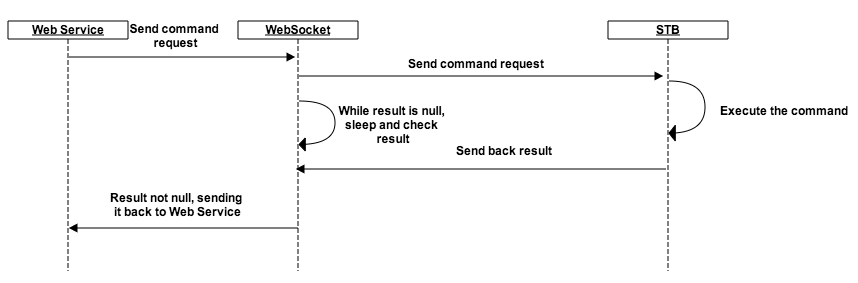
\includegraphics[width=\textwidth]{00_media/sync_data}
      \caption{Synchronisation du résultat avec le serveur}
      \label{gra:maqmenu}
\end{figure}

\subsection{Gestion de la connexion}
La gestion de la connexion consiste à garantir que peu importe les problèmes rencontrés, la connexion doit restée établie.

\medskip

\subsubsection{Serveur}
Le serveur lui doit maintenir la connexion établie en envoyant des messages. C'est son seul travail. Nous aurons donc un timer qui toutes les 5 secondes enverra un message au client.

\medskip

J'ai remarqué que lorsque la communication est interrompue, en enlevant par exemple le câble ethernet de la box, le serveur fait comme si tout se passait bien durant 60 secondes. Si la connexion est rétablie dans ce laps de temps, tout rentre dans l'ordre et les messages qui devaient être envoyés ont été bufferisés ce qui permet de les transmettre.

C'est au-delà des 60 secondes que le serveur coupe officiellement la connexion.

\begin{figure}[H]
      \centering
      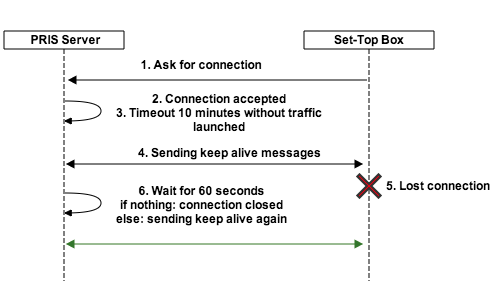
\includegraphics[width=300px]{00_media/server_ka}
      \caption{Gestion de la connexion sur le serveur}
      \label{gra:maqmenu}
\end{figure}

\subsubsection{Client}
Le client quant à lui, aura un timer de 65 secondes pour dire: "si je n'ai pas reçu de message en 65 secondes, je coupe et relance la connexion".

\medskip

Il aura un autre timer qui se connectera de manière aléatoire, entre 9 et 11 secondes, sur le serveur lorsque la connexion est perdue.
\subsection{SSL}
SSL/TLS permet de sécuriser une connexion en encryptant les données, ainsi que de certifier que le site distant est une source sûre. Dans notre cas, seule la partie de cryptage des données nous intéresse et non pas la partie certification.

\medskip

Pourtant il n'est pas facile d'avoir l'un sans l'autre et j'ai dû faire quelques modifications pour que cela fonctionne.

\medskip

Premièrement, il s'avère que Autobahn Android ne gère pas de base l'accès sécurisé \textbf{wss} du WebSocket. Cependant, une version non officielle existe. Il s'agit d'un projet à part modifier pour SSL. Pourquoi est-ce que ça n'est pas encore intégré ? Car en ajoutant la gestion de SSL, la librairie aurait perdu en rapidité de traitement des données. Donc ce n'est pas très grave dans notre cas puisque nous n'avons pas une charge excessive.

https://github.com/tavendo/AutobahnAndroid/tree/tlsnio

\medskip

Après installation sur Android, je m'occupe de Jetty. La documentation semble claire sur l'installation:

http://www.eclipse.org/jetty/documentation/current/configuring-ssl.html

Mais impossible de le faire fonctionner, une exception est levée: 

\textbf{oeji.SelectorManager:qtp1384613607-13-selector-0:}

\medskip

Et impossible de savoir de quoi cela vient. Après différents tests, c'est-à-dire refaire la configuration des clés et des certificats, essayer d'autres clients pour la connexion, toujours la même erreur.

\medskip

C'est alors que j'ai remarqué que je n'étais pas à jour avec Jetty, j'utilisais la version 9.0.3 au lieu de la 9.0.4. Mais j'utilisais les librairies de la 4! Après mise à jour, le serveur fonctionne!

\medskip

Par contre c'est à présent le client qui ne veut pas: le certification n'est pas officiellement certifié! Après quelques recherches je ne trouve pas comment palier à ce problème. Il est écrit qu'il est possible de se connecter à un serveur non certifié, mais uniquement si l'on est depuis l'émulateur Android . J'ai donc cherché où le test se faisait et ai décidé d'enlever cette condition, puis de recompilé la librairie.

\begin{lstlisting}[language=Java, caption={classe WebSocketConnection modifié}]
protected SSLContext getSSLContext() throws KeyManagementException, NoSuchAlgorithmException {
      //if (!mOptions.getVerifyCertificateAuthority()) {
         // Create a trust manager that does not validate certificate chains
         TrustManager tm = new X509TrustManager() {
            public void checkClientTrusted(X509Certificate[] chain,
                  String authType) throws CertificateException {
            }

            public void checkServerTrusted(X509Certificate[] chain,
                  String authType) throws CertificateException {
            }

            public X509Certificate[] getAcceptedIssuers() {
               return null;
            }
         };
         SSLContext ctxt = SSLContext.getInstance("TLS");
         ctxt.init(null, new TrustManager[] { tm }, null);

         Log.d(TAG, "trusting all certificates");
         return ctxt;

      // } else {
      //    Log.d(TAG, "NOT trusting all certificates");
      //    return SSLContext.getDefault();
      // }
   }
\end{lstlisting}
La partie en commentaire est l'implémentation de base.

\medskip

Ce n'est guère très propre, mais ce changement n'affecte en rien le fonctionnement de la librairie et c'était un besoin.
\section{Jersey Web Services}
Nous allons voir dans cette section comment a été installé Jersey, ainsi que son implémentation.
\subsection{Installation}
L'installation se fait via Maven. Il suffit d'ajouter les dépendances dans notre fichier \textbf{pom.xml} et de lancer la commande \textbf{mvn clean}.

\medskip

Les dépendances se trouvent sur le site officiel de Jersey.

\medskip

J'ai eu de la peine à comprendre quelles librairies utiliser au départ, car les versions ont beaucoup évoluées en peu de temps. Ainsi les exemples de configuration que l'on trouve sur Internet ne sont pas forcément à jour. Dans tous les cas, la configuration proposée est fonctionnelle en utilisation la configuration de Glassfish depuis le site de documentation cité précédemment.

\begin{lstlisting}[caption={Dépendances Maven pour Jersey}, language=XML]
<!-- Web Services -->
	<dependency>
		<groupId>org.glassfish.jersey.containers</groupId>
		<artifactId>jersey-container-servlet-core</artifactId>
		<version>2.0</version>
	</dependency>
	<dependency>
		<groupId>javax.ws.rs</groupId>
		<artifactId>javax.ws.rs-api</artifactId>
		<version>2.0</version>
		<scope>provided</scope>
	</dependency>
	<dependency>
		<groupId>org.codehaus.jackson</groupId>
		<artifactId>jackson-jaxrs</artifactId>
		<version>1.9.12</version>
	</dependency>	
  </dependencies>
\end{lstlisting}

\subsection{Hello World}

Le but de cette partie est de mettre en place un premier Web Service, qui une fois appelé nous retournerait le fameux message "Hello World"!

\medskip

Pour ce faire, il faudra définir une URL d'accès, qui sera \textbf{http://SERVER\_ADDR:8080/qosServer/rest/test/hello}. Lorsque cette adresse est atteinte, le texte "Hello World" est retourné.

Nous allons créer une classe \textbf{QOSResource} qui regroupera tous nos points d'entrée, dans le package \textbf{ch.wingo.pris.WS.resource}

\medskip

Nous devons déclarer ce package dans notre fichier \textbf{web.xml} afin de définir sous quelle URL celui-ci sera utilisée.

\begin{lstlisting}[language=XML, caption={Configuration web.xml pour Web Service}]
<servlet>
		<servlet-name>jersey-serlvet</servlet-name>
		<servlet-class>org.glassfish.jersey.servlet.ServletContainer</servlet-class>
		<init-param>
			<param-name>jersey.config.server.provider.packages</param-name>
			<param-value>ch.wingo.pris.WS.resources</param-value>
		</init-param>
	</servlet>

	<servlet-mapping>
		<servlet-name>jersey-serlvet</servlet-name>
		<url-pattern>/rest/*</url-pattern>
	</servlet-mapping>
\end{lstlisting}

Ainsi, chaque requête sur l'URL "/rest" va être redirigé dans le package "ch.wingo.pris.WS.resources".

\medskip

Voyons à présent le code Java.
\begin{lstlisting}[language=Java, caption={Implémentation Hello World Web Service}]
@Path("/test")
@Consumes(MediaType.TEXT_PLAIN)
public class QOSResource {
	
	public QOSResource(){}
	
	@Produces(MediaType.TEXT_PLAIN)
	@Path("/hello")
	@GET
	public String helloWorld(){
		return "Hello World";
	}
\end{lstlisting}
\begin{table}[H]
\begin{tabularx}{\textwidth}{|m{3cm}|X|l|}
  \hline
  \bf{Paramètre} & \bf{Description} \\
  \hline
  @Path & Permet de définir le chemin de l'URL, pour arriver au niveau de la bonne classe, puis de la bonne méthode.\\
  \hline  
  @Consumes & Définit ce qui peut être pris en paramètre des méthodes. Se met au niveau de la classe, pour une valeur par défaut, ou au niveau de la méthode, ce qui écrasera le type par défaut.\\
  \hline  
  @Produces & Définit ce qui va être produit en retour.\\
  \hline  
  @GET & Il s'agit du GET HTTP, cela veut dire que nous allons chercher une valeur. Peut donc aussi être POST, PUT ou DELETE. Une même URL peut être différencier par sa méthode HTTP!
\end{tabularx}
\caption{Résumé des paramètres Web Services}
\label{tab:classDiagram}
\end{table}

@Consumes et @Produces prennent comme valeur les différents MIME. Nous avons ici du simple texte, mais cela peut-être du JSon, du XML, du HTML etc.

\medskip

Nous avons mis comme chemin, au niveau de la classe, "/test". Donc toutes les requêtes qui contiennent "/rest/test" vont arriver ici. Ensuite la méthode helloWorld sera atteinte par l'URL "/rest/test/hello".

\subsection{Implémentation}
Chaque service aura donc une URL qui lui est propre. Le pattern suivant a été choisi:
\medskip

\textit{http://SERVER\_URL/qosServer/rest/stb/:cmd/:macAddr}

\medskip

\begin{table}[H]
\begin{tabularx}{\textwidth}{|m{3cm}|X|l|}
  \hline
  \bf{Paramètre} & \bf{Description} \\
  \hline
  /qosServer & URL de notre web application\\
  \hline  
  /rest & URL à partir de laquelle tous nos Web Services seront accessibles\\
  \hline  
  /stb & URL à partir de laquelle nous aurons accès aux Set-Top Box \\
  \hline  
  /:cmd & Ce paramètre est une variable. Sa valeur dépendra de ce que l'on veut faire. En l'occurrence, nous aurons \textbf{ping}, \textbf{iperf}, \textbf{reboot} \\
  \hline
  /:macAddr & Ce paramètre est une variable. Sa valeur sera la MAC adresse de la Set-Top Box.
\end{tabularx}
\caption{Résumé des paramètres Web Services}
\label{tab:classDiagram}
\end{table}

\medskip

Notre classe \textbf{QOSResource} sera donc implémentée. On y donnera en paramètre du JSon, pour le type de commande et les options, et le retour produit sera lui-aussi en JSon.

\begin{lstlisting}[language=Java, caption={Implémentation du Web Service}]
@Path("/stb")
//@Path("/test")
@Consumes(MediaType.APPLICATION_JSON)
public class QOSResource {
	
	public QOSResource(){}
	
	@Produces(MediaType.APPLICATION_JSON)
	@Path("/ping/{macAddr}")
	@GET
	public Response getPing(@PathParam("macAddr") String macAddr, @QueryParam("cmd") String cmd){
		System.out.println("WebService : Ping");
		String json = WebSocketsCentralisation.getInstance().ping(macAddr, cmd);
		return Response.ok(json).header("Access-Control-Allow-Origin", "*").build();
	}
	
	@Produces(MediaType.APPLICATION_JSON)
	@Path("/iperf/{macAddr}")
	@GET
	public Response getIperf(@PathParam("macAddr") String macAddr, @QueryParam("cmd") String cmd){
		System.out.println("WebService : Iperf");
		String json = WebSocketsCentralisation.getInstance().iperf(macAddr, cmd);
		return Response.ok(json).header("Access-Control-Allow-Origin", "*").build();
	}
	
	@Path("/reboot/{macAddr}")
	@GET
	public Response reboot(@PathParam("macAddr") String macAddr){
		System.out.println("WebService : Reboot");
		WebSocketsCentralisation.getInstance().reboot(macAddr);
		return Response.ok("reboot done").header("Access-Control-Allow-Origin", "*").build();
	}
	
}

\end{lstlisting}

Ce que l'on peut remarquer, c'est le retour, il s'agit d'un objet de type \textbf{Response}. Il est ainsi possible de faire un retour personnalisé en donnant un code de réponse HTML. Par exemple, si la MAC adresse est introuvable, on pourrait répondre un code 404 - not found. Le cas est ensuite traité sur la partie web, Thom. 

\medskip

Dans mon cas, il n'est pas pleinement exploité car je retourne systématiquement une réponse positive, seul le texte va changer. C'est donc un point d'amélioration possible.

\medskip

Ensuite, si je l'utilise, car nous pourrions répondre un simple String s'il est au format JSon, c'est pour le fameux problème du \textbf{Allow-origin}. En effet, il n'est \textbf{pas possible} de télécharger des données depuis un site sur un serveur. Le navigateur bloque ce genre de requête par défaut, à l'exception d'images par exemples. Il s'agit d'un système de sécurité pour éviter des intrusions.

\medskip

La solution est de réceptionner la requête, puis de modifier l'en-tête HTTP en changeant la valeur du paramètre "Access-Control-Allow-Origin". Pour l'instant, la valeur est à "*" ce qui autorise \textbf{toutes les origines}. Il serait plus judicieux de réduire au domaine hébergeant Thom afin d'améliorer la sécurité de l'application.

\medskip

Ceci est un problème que je n'avais pas prévu et qui m'a fait perdre un peu de temps.

\medskip

Autre remarque, la méthode \textbf{reboot} est à la base \textbf{void}. Lorsque cette requête est appelée, nous n'avons aucun retour sur le déroulement du redémarrage de la STB. Ceci est aussi une amélioration possible.

\medskip

Nous voyons aussi l'utilisation de notre singleton \textbf{WebSocketCentralisation}, qui regroupe les méthodes d'accès, et qui retourne le résultat de mesure.

\section{WebSocketCentralisation}

Nous allons voir comment a été implémentée cette classe centrale, élément de transition entre les Web Services et les WebSockets. Seule la méthode iperf des commandes est montrée, les autres étant similaires.
\subsection{Implémentation}
\begin{lstlisting}[language=Java,caption{Implémentation de WebSocketCentralisation}]
	// singleton of websocketcentralisation
	private static final WebSocketsCentralisation INSTANCE = new WebSocketsCentralisation();
	// HashMap regrouping all the sessions, identifiable by the MAC Addr
	private HashMap<String, RemoteSTBSocket> members = new HashMap<String, RemoteSTBSocket>();
	// Constant value if no user is found in members
	private static final String USER_NOT_FOUND = "{\"error\":\"user not found\"}";
	
	public static WebSocketsCentralisation getInstance(){
		return INSTANCE;
	}
	
	// Join: Add the session to the HashTable
	public void join(RemoteSTBSocket socket){
		System.out.println(new Date()+" New socket connexion added: "+socket.getMacAddr());
		// adding the socket to the hashtable
		members.put(socket.getMacAddr(), socket);
		// printing the connected boxes
		for(RemoteSTBSocket sockets:members.values()){
			System.out.println(new Date()+" Is connected: "+sockets.getMacAddr());
		}
	}
	
	// Leave: Remove the session from the HashTable
	public void leave(RemoteSTBSocket socket){
		System.out.println(new Date()+" Socket connexion removed: "+socket.getMacAddr());
		// removing the socket from the hashtable
		members.remove(socket.getMacAddr());
		// printing the connected boxes
		for(RemoteSTBSocket sockets:members.values()){
			System.out.println(new Date()+" Is connected: "+sockets.getMacAddr());
		}
	}
	
	// Will ask the correct Session to iperf
	public String iperf(String macAddr, String cmd) {
		// if the session exists
		if(members.containsKey(macAddr))
			// returning the iperf value from the session
			return members.get(macAddr).iperf(cmd);
		// else returning error message
		else return USER_NOT_FOUND;
	}
\end{lstlisting}

On retrouve donc les éléments expliqués, une HashTable regroupant toutes nos connexions, les méthodes "join" et "leave" permettant de rejoindre et de quitter la HashTable, ainsi qu'une méthode de commande, iperf.

\medskip

Celle-ci va donc récupérer la bonne session grâce à la MAC adresse, exécuter la commande iperf de la session et attend le résultat. Nous verrons à la prochaine étape comment se fait "l'attente".

\section{RemoteSTBSocket}
Voici la partie traitant de la communication par les WebSockets. Il s'agit de voir comment les requêtes sont envoyées, réceptionnées et comment la connexion est gérée.

\subsection{Traitement des requêtes}
Dans la classe WebSocketCentralisation, nous avons vu que nous utilisions la méthode "iperf" des websockets. Son but est d'envoyer un message via la session à la STB, et d'attendre le résultat pour le retourner.

\begin{lstlisting}[language=Java, caption={Méthode iperf du WebSocket}]
// sending iperf request to the stb
	// waiting for the result
	// called by WebSocketCentralisation
	public String iperf(String cmd) {
		String result = ""; // result sends back
		// send command to the stb via websocket
		session.getRemote().sendStringByFuture(cmd);
		try{
			System.out.println(new Date()+ " Gonna wait");
			// while the iperf result is empty
			while (iperfResult.equals("")) {
				// I sleep for 10 ms
				Thread.sleep(10);
			}
		} catch(InterruptedException e){
			e.printStackTrace();
		}
		// if i m out, i have a result! Copying the iperResult
		result = iperfResult;
		// reinitialising iperfResult for next time
		iperfResult = "";
		System.out.println(new Date()+" No more sleeping, gonna send: "+result);
		// returning the result to WebSocketCentralisation
		return result;
	}
\end{lstlisting}

Nous voyons que la méthode \textbf{attend} le résultat du String \textbf{iperfResult}. Cet objet est mis à jour lors de la réception du résultat envoyé par la STB. Nous allons justement voir comment cela se passe.

\begin{lstlisting}[language=Java, caption={Réception d'un retour de résultat STB to PRIS}]
@OnWebSocketMessage
    public void onText(Session session, String message) {
        if (session.isOpen()) {
ObjectMapper mapper = new ObjectMapper(); // mapper to convert a String JSon to a map
			Map<String, Object> map; // map containing the result json in format key/value
			try {
				// converting the String json to a map
				map = mapper.readValue(message, new TypeReference<Map<String, Object>>() {});
				// getting the type of command
				String type = (String) map.get("type");
				 if(type.equals("iperf")){
					System.out.println(new Date()+" Socket: iperf result received");
					// updating iperfResult with message, the result.
					// the sleeping thread will now awake!
					iperfResult = message;
				} 
			}
\end{lstlisting}

Lorsque le résultat est reçu, nous testons s'il s'agit d'iperf. Si c'est le cas, nous allons mettre à jour "iperfResult". Il s'agit d'objet dont le Thread attend le changement de valeur pour le renvoyer. Nous sommes ainsi notifiés de manière très rapide.

\subsection{Gestion de la connexion}
Pour la partie serveur, la gestion de la connexion se limite à envoyer des \textbf{Keep Alive}. Ceci se fait via un Timer, qui toutes les \textbf{SEND\_KEEP\_ALIVE\_MS}, va envoyer un message en disant simplement \textbf{hello}.

\begin{lstlisting}[language=Java, caption={Code de lancement des Keep Alive}]
@OnWebSocketConnect
	public void onConnect(Session session){
		System.out.println(new Date()+" Device connected: "+session.getRemoteAddress().getHostString());
		keepAliveTimer.schedule(new KeepAliveTask(), 0, SEND_KEEP_ALIVE_MS);
		this.session = session;
	}
	
	// Task for timer to send hello messages to maintain 
	// the connexion
	private class KeepAliveTask extends TimerTask{
		
		@Override
		public void run() {
			session.getRemote().sendStringByFuture("hello");
		}
	}
\end{lstlisting}

L'utilisation de la méthode \textbf{sendStringByFuture}, qui rappelons-le, est \textbf{non bloquante}, est dans ce cas pratique puisque déjà, un nouveau thread est créé pour juste envoyer les messages, et en plus il peut le faire de manière continu. Ce n'est pas dit que toutes les 5 secondes la STB reçoive le message, mais au moins ceux-ci sont empilés et seront de toute façon envoyés.

\medskip

Comme expliqué, c'est après un décompte de 60 secondes, que le serveur va stopper définitivement la connexion. Nous rentrons dans la méthode "onClose" qui va me permettre de bien vérifier que toute connexion soit arrêtée, puis de quitter la HashTable de la classe "WebSocketCentralisation".

\medskip

Lorsque c'est le serveur qui reçoit à son tour un message \textbf{hello} de la part de la STB, il n'y a rien que l'on puisse faire puis que le décompte sans communication se fait au niveau du client.

\begin{lstlisting}[language=Java, caption={Réception d'un keep alive sur le serveur}]
if(message.equals("hello")){
	return;
}
\end{lstlisting}

\subsection{Premier message reçu}
Le premier message que le serveur reçoit, ce doit être la MAC adresse de la Set-Top Box. Nous allons donc vérifier qu'il s'agisse bien de cela puis si tel est le cas, nous enregistrer auprès de la classe "WebSocketCentralisation".

\begin{lstlisting}[language=Java, caption={Code d'enregistrement de la Set-Top Box}]
@OnWebSocketMessage
    public void onText(Session session, String message) {
        if (session.isOpen()) {
        	if(firstConnection && isMacAddr(message)){
        		System.out.println(new Date()+" First message: should be mac addr: "+message);
        		firstConnection = false;
        		this.macAddr = message;
        		WebSocketsCentralisation.getInstance().join(this);
        		return;
        	}
\end{lstlisting}

\section{AutoStartService sur Android}
Voici la partie Android. Certaines choses ont déjà été vues, les implémentations du ping et de iperf, ainsi que la connexion au serveur.

Nous allons voir comment se passe l'initialisation de la connexion, la réception de message, comment convertir un objet java en Json et surtout la gestion de la connexion du côté client, qui a la tâche de vérifier la réception des keep alive et de se reconnecter en cas de problème.

\subsection{Première message}
Le premier message envoyé par la box doit être sa MAC adresse. Il faut pour cela la récupérer et nous aurons besoin de savoir quelle interface est active sur la Set-Top Box. Pour le moment, seule la connexion via ethernet est possible, mais le code a été fait en sorte de supporter la connexion Wifi aussi.

Les interfaces sont listables via la commande \textbf{adb shell netcfg}

\medskip

Ces méthodes font partie de la classe statique \textbf{NetworkUtils} qui me permet à tout moment de récupérer ses informations d'informations.

\begin{lstlisting}[language=Java, caption={Network Utils}]
public static String getActiveInterface(Context context){
		ConnectivityManager cm = (ConnectivityManager) context.getSystemService(Context.CONNECTIVITY_SERVICE);
		switch (cm.getActiveNetworkInfo().getType()) {
		case ConnectivityManager.TYPE_ETHERNET:
			return "eth0";
		case ConnectivityManager.TYPE_WIFI:
			return "ra0";

		default:
			break;
		}
		return null;
	}
	
		// return the MAC address of the device
	public static String getMACAddr(String interfaceName) {
		try {
			// getting all the interfaces
			List<NetworkInterface> interfaces = Collections
					.list(NetworkInterface.getNetworkInterfaces());
			
			for (NetworkInterface intf : interfaces) {
				if (interfaceName != null) {
					// checking that the interface given exists
					if (!intf.getName().equalsIgnoreCase(interfaceName))
						continue;
				}
				// getting the mac address on byte array format
				byte[] mac = intf.getHardwareAddress();
				if (mac == null)
					return "";
				StringBuilder buf = new StringBuilder();
				// converting byte array to readable String
				for (int idx = 0; idx < mac.length; idx++)
					buf.append(String.format("%02X:", mac[idx]));
				if (buf.length() > 0)
					buf.deleteCharAt(buf.length() - 1);
				return buf.toString();
			}
		} catch (Exception ex) {
			Log.e(TAG, ex.toString());
		}
		return "";
	}
\end{lstlisting}
La méthode getMACAddr a été trouvée sur StackOverFlow

http://stackoverflow.com/questions/14190602/how-to-get-the-mac-address-of-an-android-devicewifi-is-switched-off-through-co

\medskip

Maintenant que la mac adresse est récupérée, nous pouvons l'envoyer au serveur.

\begin{lstlisting}[language=Java, caption={Envoi de la mac adresse au serveur}]
// when the connexion is established
				@Override
				public void onOpen(){
					Log.d(TAG, "Connected");
					Log.d(TAG, "First connexion, sending MAC @");
					Log.d(TAG, "My MAC Addr: "+ macAddr);
					mConnection.sendTextMessage(macAddr);
				}
\end{lstlisting}
\subsection{Traitement des requêtes}
Cela se passe à la méthode \textbf{onTextMessage}, à la réception d'un message. Lorsqu'il y a des options, comme avec ping et iperf, on réceptionne du JSon, et celui-ci commence toujours par le caractère \textbf{\{}.

Autrement nous recevrons des String. Pour les commandes qui ne demandent pas d'option particulière (reboot) et pour les message de \textbf{Keep Alive} (hello).

\begin{lstlisting}[language=Java, caption={Réception d'une commande avec options}]
@Override
		         public void onTextMessage(String payload) {
		            Log.d(TAG, "Message received: "+payload);
		            // if we have JSon
		            if(payload.startsWith("{")){
		            	ObjectMapper mapper = new ObjectMapper(); // mapper String Json to map
		            	Map<String, Object> map; // map key/value of the json recept
		            	try {
		            		// converting the string to map
							map = mapper.readValue(payload, new TypeReference<Map<String, Object>>() {});
							// if we have a an iperf
							if(map.get("cmd").equals("iperf")){
								Log.d(TAG, "Iperf request received");
								// we get des options of the command
								String opt = (String) map.get("opt");
								// mapper Java Object to JSon
								ObjectMapper toJson = new ObjectMapper();
								// the result sent back
								String json = "";
								try {
									// IperResult instantiate feed!
									IperfResult ir = iperf(opt);
									// if everything was good:
									if(ir != null){
										json = toJson.writerWithDefaultPrettyPrinter().writeValueAsString(ir);
									}
									// else the iperf server was certainly down. Creating a new JSon.
									else {
										JSONObject job = new JSONObject();
										job.put("message", "Error during iperf. Check if iperf server is up!");
										job.put("type", "error");
										job.put("command", "iperf");
										// make it pretty, not in a single line
										json = job.toString(2);
									}
									
								} catch (JsonGenerationException e) {
									e.printStackTrace();
								} catch (JsonMappingException e) {
									e.printStackTrace();
								} catch (IOException e) {
									e.printStackTrace();
								} catch (JSONException e) {
									e.printStackTrace();
								}
								// sending back the result to the server
								mConnection.sendTextMessage(json);
							}
						}
\end{lstlisting}

La \textbf{ligne 25} est intéressante. Car cette fois, au lieu d'utiliser un mapper pour convertir un String en map, nous convertissons un \textbf{objet java} en String sous format JSon. Regardons de plus près la classe \textbf{IperfResult}.

\begin{lstlisting}[language=Java, caption={classe IperfResult}]
public class IperfResult {
	private String type;
	private String macAddr;
	private double throughput;
	private String unit;
	
	public IperfResult(){}
	
	public IperfResult(String type, String macAddr, double throughput, String unit){
		this.type = type;
		this.macAddr = macAddr;
		this.throughput = throughput;
		this.unit = unit;
	}
	
	public String getType() {
		return type;
	}
	public void setType(String type) {
		this.type = type;
	}
	public String getMacAddr() {
		return macAddr;
	}
	public void setMacAddr(String macAddr) {
		this.macAddr = macAddr;
	}
	public double getThroughput() {
		return throughput;
	}
	public void setThroughput(double throughput) {
		this.throughput = throughput;
	}
	public String getUnit() {
		return unit;
	}
	public void setUnit(String unit) {
		this.unit = unit;
	}
}
\end{lstlisting}
Ce que l'on peut remarquer, c'est que chaque attribut possède un \textbf{get} et un \textbf{set} portant son nom. Ceci est une règle pour pouvoir convertir un objet directement en JSon. Ainsi que de posséder un constructeur vide.

\medskip

Nous allons voir comment parser le résultat d'iperf, qui est un flux de String. Nous allons utiliser pour cela les expressions régulières.
\begin{lstlisting}[language=Java, caption={Parsing du résultat d'une commande Iperf}]
String str1 = ""; // will contain each line
			String[] arrayOfString = null; // will contain the results
			while ((str1 = reader.readLine()) != null) {
				Log.d(TAG, "Entering iperf result process");
				// regex for a line with our result. We double de \ in java
				if (str1.matches("\\[[ \\d]+\\]\\s*[\\d]+.*")) {
					Log.d(TAG, "We got a match, filtering...");
					// regex for the between of each value
					Pattern localPattern = Pattern.compile("[-\\[\\]\\s]+");
					// we split the line with our pattern. We get the results
					arrayOfString = localPattern.split(str1);
					break;
				}
				// regex to catch if the server it down
				if (str1.matches("[a-zC:\\s]+")) {
					Log.d(TAG, "Connection refused - no server found");
					reader.close();
					process.destroy();
					return null;
				}
			}
\end{lstlisting}

Nous avons une première expression, qui permet de récupérer la ligne contenant les données de résultat.
\begin{figure}[H]
      \centering
      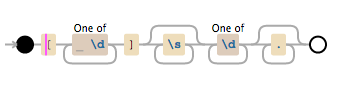
\includegraphics[width=300px]{00_media/regex_line_match_sch}
      \caption{Expression régulière pour la ligne de résultat}
      \label{gra:maqmenu}
\end{figure}
 
\begin{figure}[H]
      \centering
      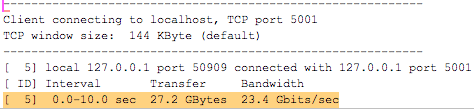
\includegraphics[width=320px]{00_media/regex_line_match}
      \caption{Vu de la ligne de résultat}
      \label{gra:maqmenu}
\end{figure}

En ce qui concerne le split entre les valeurs:
\begin{figure}[H]
      \centering
      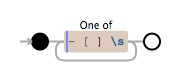
\includegraphics[width=150px]{00_media/regex_between_value_sch}
      \caption{Expression régulière pour la ligne de résultat}
      \label{gra:maqmenu}
\end{figure}
 
\begin{figure}[H]
      \centering
      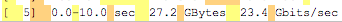
\includegraphics[width=220px]{00_media/regex_between_value}
      \caption{Vu de la ligne de résultat}
      \label{gra:maqmenu}
\end{figure}

Donc tous les entre-valeurs que l'on désire récupérer sont interceptés. Lorsque l'on split la ligne, nous aurons un tableau de valeurs. Il suffit d'instancier un objet IperfResult, de lui donner les valeurs, et de le retourner pour qu'il soit converti en JSon.

\subsubsection{Reboot}
Voici l'implémentation du reboot sous Android. Il nécessite la permission \textbf{<uses-permission android:name="android.permission.REBOOT" />} à ajouter dans le fichier \textbf{AndroidManifest.xml}, qui nécessite d'être \textbf{root} pour l'exécuter.

\begin{lstlisting}[language=Java, caption={Code du reboot}]
private void reboot() {	((PowerManager)STBContext.getAppContext().getSystemService(Context.POWER_SERVICE)).reboot(null);
	}
\end{lstlisting}

Nous récupérons une instance de \textbf{PowerManager} qui permet, comme son nom l'indique de gérer l'énergie du terminal sous Android. Toutefois attention:

\begin{shadequote}
Device battery life will be significantly affected by the use of this API
\par\emph{Tiré de la documentation officielle d'Android}
\end{shadequote}

Mais notre STB est sous alimentation nous n'avons donc pas de soucis à nous faire.

http://developer.android.com/reference/android/os/PowerManager.html
\subsection{Gestion de la connexion}
Pour cette section, nous avons deux parties.
\begin{enumerate}
	\item Une partie permettant de vérifier que nous avons bien reçu les keep alive
	\item Une partie permettant de se reconnecter au serveur en cas de problème
\end{enumerate}
\subsubsection{Keep Alive}

Chaque fois que l'on va recevoir un message "hello" du serveur, un Timer nommé \textbf{timeWithoutMessage} va être déclenché. Du côté serveur, la connexion est rompue au bout de 60 secondes s'il y a un problème de connexion. Ici, nous allons donc donné 65 secondes au Timer. Si au bout de 65 secondes aucun message n'a été réceptionné, alors le Timer permettant de se reconnecter au serveur va être déclenché.

\medskip

Le timer est lancé dès la connexion. Ensuite, si je reçois un message "hello", je peux annuler le timer, réceptionner le message et renvoyer un "hello" au serveur, et relancer le timer.

\begin{lstlisting}[language=Java, caption={Code Keep Alive Android}]
	if(payload.equals("hello")){
		// cancelling the timer
		tt.cancel();
		timeWithoutMessage.purge();
		// sending hello back to the server
		mConnection.sendTextMessage(payload);
		// lauching the timer again
		tt = createTimeWithoutMessageTask();
		timeWithoutMessage.schedule(tt, WAIT_WITHOUT_MESSAGE);
	}
	// when de 65 secondes are done
	private TimerTask createTimeWithoutMessageTask(){
		return new TimerTask() {
			@Override
			public void run() {
				Log.d(TAG, "Waiting for a minute, trying de reconnect");
				mConnection.disconnect();
				reconnectToServer();
			}
		};
	}
\end{lstlisting}

Lorsque les 65 secondes sont écoulées, le Timer exécute sa méthode run, qui va se déconnecter du serveur afin de mieux s'y reconnecter!

\subsubsection{Ping/Pong frames}
Le protocole des WebSockets spécifient que l'on peut utiliser les frames Ping et Pong pour maintenant la connexion client serveur. Le ping est envoyé depuis le serveur, via la command \textbf{sendPingFrame}, et la librairie Autobahn va automatiquement répondre par un Pong pour confirmer qu'on est toujours là. Ce sont d'ailleurs ces requêtes qui sont utilisés par Jetty pour calculer les fameux 10 minutes de connexion.

\medskip

Le problème est que nous n'avons aucun contrôle sur le Ping reçu sur Android. En effet, c'est la librairie qui gère cela sans proposer de méthode de réception à l'instar de \textbf{onTextMessage}. J'étais au début parti sur cette voie, qui fonctionnait jusqu'à un certain point, puisque je ne pouvais pas calculer combien de temps s'écoulait entre les réceptions de Ping.

\medskip

La gestion du Ping/Pong sur Autobahn est une requête demandée par les utilisateurs. Si le temps m'en avait permis, j'aurais pu me pencher sur ce cas afin d'une part l'utiliser dans mon projet et d'autre par contribuer au projet open source de cette librairie. Mais j'ai privilégié l'alternative qui consistait à implémenter moi-même la solution de keep alive.

https://github.com/tavendo/AutobahnAndroid/issues/31
\subsubsection{Reconnexion au serveur}
La reconnexion se lance depuis deux situations:
\begin{enumerate}
	\item Lorsque la connexion est correctement fermée. Ici, nous rentrons dans l'événement \textbf{onClose}
	\item Lorsque la connexion n'est pas correctement fermée. Dans ce cas, c'est le timer des keep alive qui va relancer la connexion.
\end{enumerate}

Lorsque la connexion se passe bien, par exemple si le serveur est arrêté et que la fin de connexion WebSocket est faite correctement, nous passons par la méthode \textbf{onClose} proposée par la librairie.

\begin{lstlisting}[language=Java, caption={Code onClose Android}]
    @Override
		         public void onClose(int code, String reason) {
		            Log.d(TAG, "Connection lost. "+reason+" error code : "+code);
		            // under 4000 it is managed by the library.
		            // we can custom our own codes if we want
		            if(code<4000){
		            	reconnectToServer();
		            }
		         }
\end{lstlisting}

La particularité, c'est que si l'on passe dans \textbf{onClose}, la connexion est déjà interrompue. Et si l'on essaie de se reconnecter directement, on repasse dans le onClose! Ce qui fait une boucle infinie et tue l'application. C'est une particularité de Autobahn, qui à mes yeux ne fait pas tellement sens. Si la connexion n'existe plus, pourquoi retombe-t-on dans onClose? En tout cas je n'avais pas tout de suite compris cela, ce qui m'a fait perdre passablement de temps. Pour contrer ce problème, j'utilise un boolean \textbf{goConnect}, qui est initialisé à \textbf{true}. Lorsqu'on tente de se reconnecter pour la première fois, on est autorisé. Puis l'on change le boolean à \textbf{false}, pour éviter la boucle infini, qui ne lancera ainsi le timer qu'une seule fois.

\begin{lstlisting}[language=Java, caption={Code de reconnexion au serveur}]
private void reconnectToServer() {
		try {
			// boolean to check that the task is launched
			// only one time
			if(goConnect){
				goConnect = false;
				Thread.sleep(1000);
				Log.d(TAG, "ReconnectTimer Launched");
				// launching the Task
				new ReconnectTask().run();
			}
		} catch (InterruptedException e) {
			e.printStackTrace();
		}
		
	}
		// task launching one time, when connetion is lost
	private class ReconnectTask extends TimerTask{
		@Override
		public void run() {
			try{
				// if we don t wait for an hour
				if(totalWaitTime<HOUR_TO_MS){
					// if we are still deconnected
					if(!mConnection.isConnected()){
						// random waiting time between a min and max value
						int waitTime= random.nextInt(MAX_TO_WAIT - MIN_TO_WAIT + 1) + MIN_TO_WAIT;
						Log.d(TAG, "Next tentative to connect in "+waitTime+" ms");
						// calculate the total waiting time
						totalWaitTime +=waitTime;
						// schedule a new reconnection waitTime later
						reconnectTimer.schedule(new ReconnectTask(), waitTime);
						// trying to connect
						connectToServer();
					}else{
						// if the task was launched but we are connected now
						Log.d(TAG, "Connected to the server again");
						// reinitializing parameters for next interruption
						reinitializeReconnection();
					}
				}else throw new InterruptedException("Attempt to connect to the server during 1 hours without success");
			}catch(InterruptedException e){
				Log.d(TAG, e.getMessage());
			}
		}
		
	}
\end{lstlisting}

J'ai décidé que c'était la Task elle-même qui allait lancer le timer. Pourquoi ? Car nous avons un \textbf{temps aléatoire}. Or, il est impossible de base de lancer le timer de manière aléatoire. Nous devons lui donner des temps fixes.

L'autre avantage est que je n'ai qu'une seule instance de \textbf{ReconnectTask}, ce qui me permet d'avoir des variables à travers les différentes tentatives de connexion, typiquement \textbf{totalWaitTime} qui va accumuler tout le temps attendu, jusqu'à atteindre une heure de reconnexion.